%\documentclass{article}
%\usepackage{tikz,pgfplots}
%\usepackage[pdftex,active,tightpage]{preview}
%\begin{document}
%\begin{preview}
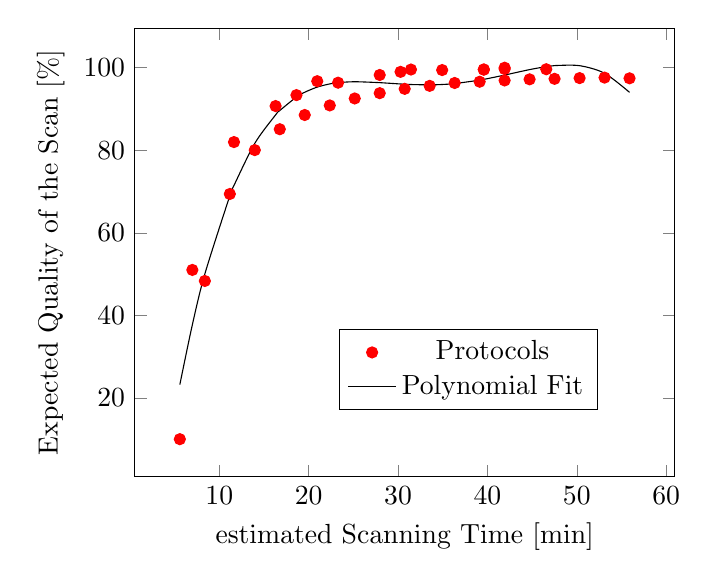
\begin{tikzpicture}
\begin{axis}[%
%	width=\linewidth,%
	xlabel={estimated Scanning Time [min]},%
	ylabel={Expected Quality of the Scan [\%]},%
	]

% Line plot
\addplot [ color = red, only marks, mark = *] 
coordinates{
 (5.5875,10) (6.98958,51.0063) (8.3875,48.3324) (11.1813,69.4075) (11.6458,81.985) (13.975,80.0399) (16.3021,90.7093) (16.7688,85.096) (18.6354,93.3621) (19.5625,88.5423) (20.9625,96.7319) (22.3625,90.8617) (23.2917,96.3704) (25.1563,92.5481) (27.9479,98.2413) (27.95,93.8354) (30.2813,98.9979) (30.7437,94.8773) (31.4438,99.5581) (33.5375,95.6051) (34.9375,99.4314) (36.3375,96.2983) (39.1313,96.6062) (39.5938,99.5875) (39.5958,99.5241) (41.925,100) (41.925,96.9138) (41.9271,99.6929) (44.7188,97.1848) (46.5833,99.6309) (47.5125,97.3067) (50.3125,97.4836) (53.1063,97.603) (55.9,97.4336)
};

% Line plot
\addplot [ smooth ] 
coordinates{
 (5.5875,23.213) (6.98958,37.7379) (8.3875,50.0404) (11.1813,68.9695) (11.6458,71.4736) (13.975,81.6837) (16.3021,88.5733) (16.7688,89.6234) (18.6354,92.9028) (19.5625,94.0559) (20.9625,95.3079) (22.3625,96.078) (23.2917,96.3777) (25.1563,96.6032) (27.9479,96.3862) (27.95,96.3859) (30.2813,96.0569) (30.7437,96.0006) (31.4438,95.9286) (33.5375,95.8484) (34.9375,95.9383) (36.3375,96.1591) (39.1313,96.986) (39.5938,97.167) (39.5958,97.1679) (41.925,98.211) (41.925,98.211) (41.9271,98.212) (44.7188,99.5426) (46.5833,100.268) (47.5125,100.516) (50.3125,100.492) (53.1063,98.6574) (55.9,94.0299)
};

\pgfplotsset{every axis legend/.append style={
at={(0.618,0.2)},
anchor=base}}

\legend{Protocols,Polynomial Fit}%$p(x)=p_{1}x^{n}+p_{2}x^{n-1}+...+p_{n}x+p_{n+1}$}

\end{axis}
\end{tikzpicture}
%\end{preview}
%\end{document}